\begin{frame}{Lecturers' introduction}
\lcol
\begin{singlespace}
%
\begin{figure}
\centering

\includegraphics[height=0.6\columnwidth]{figures/intro/logo-kyas}
\caption*{Dr. Svetlana Kyas, Post-Doctoral Associate in Geothermal Energy \& Geofluids}
\end{figure}
%
\end{singlespace}
%
\rcol
\begin{figure}
\vskip 5pt
\centering

\includegraphics[height=0.6\columnwidth]{figures/intro/logo-leal.jpg}
\caption*{Dr. Allan Leal, Senior Research Assistant in Geothermal Energy \& Geofluids}
\end{figure}
\ecol
  
\end{frame}

\section[Introduction]{Introduction}

\subsection[Course introduction]{Course introduction}

% --------------------------------------------------------------------------------------------------------------------%
% Outline
% --------------------------------------------------------------------------------------------------------------------%
\begin{frame}{Course goal}
\vskip 10pt
\begin{itemize}
\item By the end of this course, you should become familiar with the fundamentals
of \textbf{geochemical and reactive transport modeling} that includes of the following concepts: 
\begin{itemize}
\item chemical equilibrium;
\item chemical kinetics; and
\item chemical transport.
\end{itemize}
\pause
\item For \textbf{numerical simulations} of simple geochemical and reactive transport problems, 
we will use Python and Reaktoro (\href{https://reaktoro.org/}{\textcolor{indigo(dye)}{\tt reaktoro.org}}, computational framework that provides numerical methods for modeling chemically reactive processes governed by either chemical equilibrium, chemical kinetics, etc).
\end{itemize}

\begin{figure}
\centering

\includegraphics[height=0.15\columnwidth]{figures/intro/logo-python.png}

\includegraphics[height=0.15\columnwidth]{figures/intro/logo-reaktoro.png}
\end{figure}

\end{frame}

% --------------------------------------------------------------------------------------------------------------------%
% Computational Project
% --------------------------------------------------------------------------------------------------------------------%
\begin{frame}{Computational exercises}
\small

\begin{itemize}
\item This course will include a \alert{\textbf{computational project}} using Python, Jupyter Notebook, and possibly Git:
%
\begin{itemize}
\item The project \textbf{is graded} and helpful if you want to get the experience and improve you final grade. But \textbf{not necessary}. 
\pause
Possible forms of the project: 
\begin{itemize}
\item learning basics of geochemical simulation on one example (dissolving calcite in CO2-rich brine) in Python, 
\item learning Reaktoro (Python-based framework to model geochemical reactions) via doing hands-on Jupyter notebook exercises (on variety of problems), or 
\item learning Reaktoro via Jupyter notebooks and by trying to model and program realistic application example (try out a new interesting application). 
\end{itemize}
% \item It will involve chemical reaction calculations for a \textbf{chemical system} containing different 
% phases, such as 
% %
% \begin{itemize}
% \item aqueous (HO$_2$(l), HCl(aq), Na$^+$, etc), 
% \item gaseous (CO$_{2}$(g), H$_{2}$S(g)), and 
% \item mineral (e.g., calcite, dolomite, halite). 
% \end{itemize}
% \pause
% \item The goal of these calculations can be, for example, to determine the solubility
% of minerals and gases in saline waters (brine) at different salinities,
% temperatures, and pressures. 
%\pause
%\item You are welcome to team up to complete this project. 
% \pause
% \item \textbf{Optional}: We can select the time (to meet online) so that you get to ask your questions, 
% and I will be able to clarify them. 
\end{itemize}
\pause
\item Other computational tasks will be given throughout the lectures as \alert{\textbf{exercises, code-listings, and tutorials}} (using python scripts or Jupyter Notebooks).
%
\pause
\item Lectures will contain \alert{\textbf{interactive quizzes}} helping to understand and apply the presented material. 
%
\begin{center}
    LET'S TRY THE QUIZZES OUT!
\end{center}
\end{itemize}
%\pause
%\alert{\textbf{Note}}: A document detailing the project's computational assignment will be shared with you later.
\end{frame}


% --------------------------------------------------------------------------------------------------------------------%
% Learning Python
% --------------------------------------------------------------------------------------------------------------------%

\begin{frame}{Poll on the you background and preferences}
\centering 
\vskip 10pt
{\Large \href{http://etc.ch/M2Rp}{\textcolor{indigo(dye)}{\tt http://etc.ch/M2Rp}}}\\ 
or \\[10pt]

\includegraphics[height=0.4\columnwidth]{figures/intro/poll.png}
\end{frame}


% --------------------------------------------------------------------------------------------------------------------%
% Learning Python
% --------------------------------------------------------------------------------------------------------------------%
\begin{frame}{Tips for learning}
\begin{itemize}
\item It is sufficient to learn the \alert{\textbf{basics of the Python 3}} using
\end{itemize}
\begin{center}
{\href{https://www.programiz.com/python-programming/tutorial}{\textcolor{indigo(dye)}{\tt https://www.programiz.com/python-programming/tutorial}}}{\large\par}
\par\end{center}
\begin{itemize}
\item \alert{\textbf{Git}} intro
\end{itemize}
\begin{center}
{\href{https://youtu.be/hwP7WQkmECE}{\textcolor{indigo(dye)}{\tt https://youtu.be/hwP7WQkmECE}}}{\large\par}
\par\end{center}
\begin{itemize}
\item Consider installing Python 3 using \alert{\textbf{Anaconda}} using
\end{itemize}
\begin{center}
{\href{https://www.anaconda.com/distribution/}{\textcolor{indigo(dye)}{\tt https://www.anaconda.com/distribution/}}}{\large\par}
\par\end{center}
\begin{itemize}
\item Instruction of \alert{\textbf{installing Reaktoro}} are also given using Anaconda are given in videos 
\emph{Intro words}, 
\emph{Installation on Windows / IoS}, and 
\emph{Reaktoro Jyputer Notebook Installation} with explanation on Reaktoro installation and Jupyter Notebook tutorials execution are available \href{https://polybox.ethz.ch/index.php/s/qStBnxUnry648U5}{\textcolor{indigo(dye)}{\it here}}. 
%
\item 
Questions are always welcome via my email \href{svetlana.kyas@erdw.ethz.ch}{\textcolor{indigo(dye)}{\tt svetlana.kyas@erdw.ethz.ch}}. 
%or the \href{https://gitter.im/geofluids/community}{\textcolor{indigo(dye)}{\it Gitter chat}} (requires the github account).
\end{itemize}

\end{frame}
% --------------------------------------------------------------------------------------------------------------------%
% Example of geochemical calculations
% --------------------------------------------------------------------------------------------------------------------%
\begin{frame}{Example of geochemical calculations, CO$_2$(g) solubility in the NaCl-brine}
\vskip 10pt
\Wider{
\begin{figure}
\centering
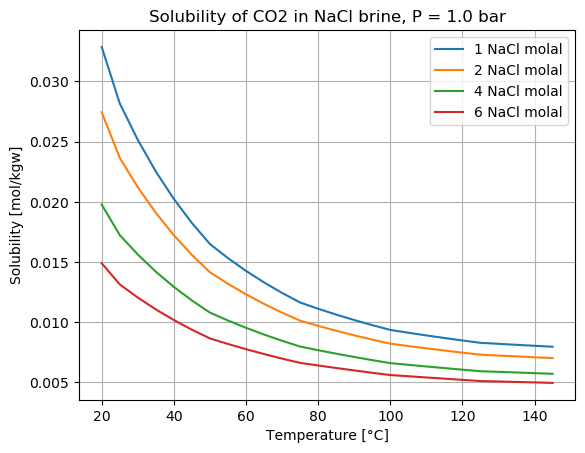
\includegraphics[height=0.37\columnwidth]{figures/intro/co2-solubility-nacl-h2o-1bar.png}
%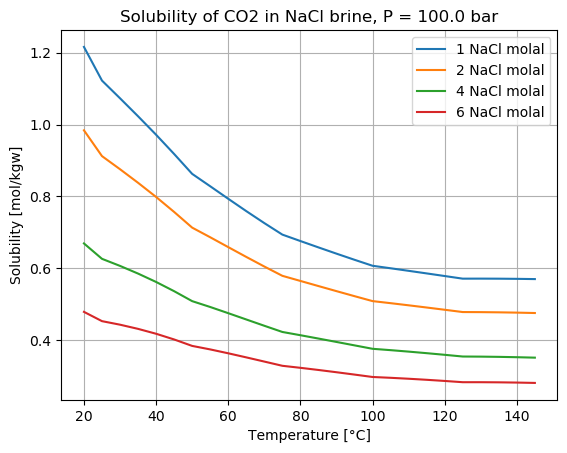
\includegraphics[height=0.3\columnwidth]{figures/intro/co2-solubility-nacl-h2o-100bar.png}\\
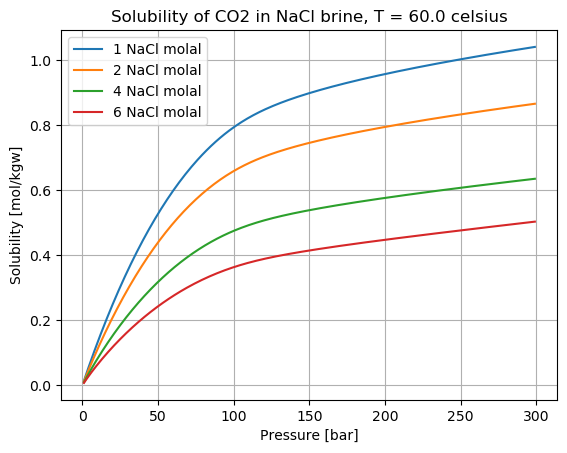
\includegraphics[height=0.37\columnwidth]{figures/intro/co2-solubility-nacl-h2o-vs-pressure-60celsius.png}
%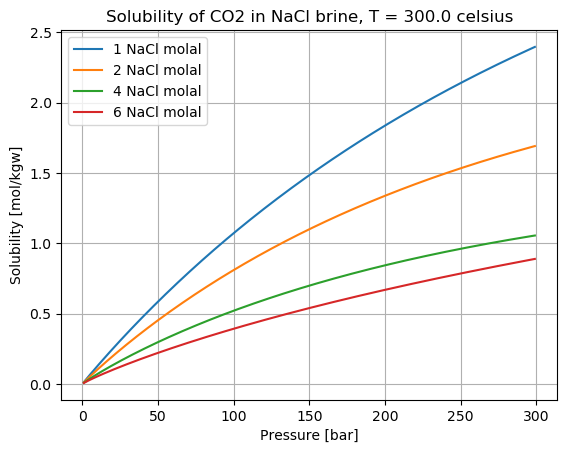
\includegraphics[height=0.3\columnwidth]{figures/intro/co2-solubility-nacl-h2o-vs-pressure-300celsius.png}
\end{figure}
}
\vskip 10pt
{\bf Note}: See \href{https://reaktoro.org/applications/solubility/solubility-co2-on-salinity-and-temperature.html}{\textcolor{indigo(dye)}{\it Reaktoro v2.0 example}} with the \href{https://github.com/mtsveta/reaktoro-v2-workshop/blob/main/tutorials/applications/salting-out-effect-co2.ipynb}{\textcolor{indigo(dye)}{\it Jupyter notebook}}.

\end{frame}

% --------------------------------------------------------------------------------------------------------------------%
% A brief overview of geochemical modeling and its applications
% --------------------------------------------------------------------------------------------------------------------%
%
\subsection{A brief overview of geochemical modeling and its applications}
           %A brief overview of geochemical modeling and its applications
\begin{frame}{What is geochemical modeling?}
\vskip 10pt
 \textbf{Geochemical modeling} is the use of computers to simulate \textbf{chemical
reactions} occurring in geologic systems, either \textbf{near the
Earth's surface} or \textbf{deep in its interior}.
%
\lcol
\begin{singlespace}
%
\begin{figure}
\centering
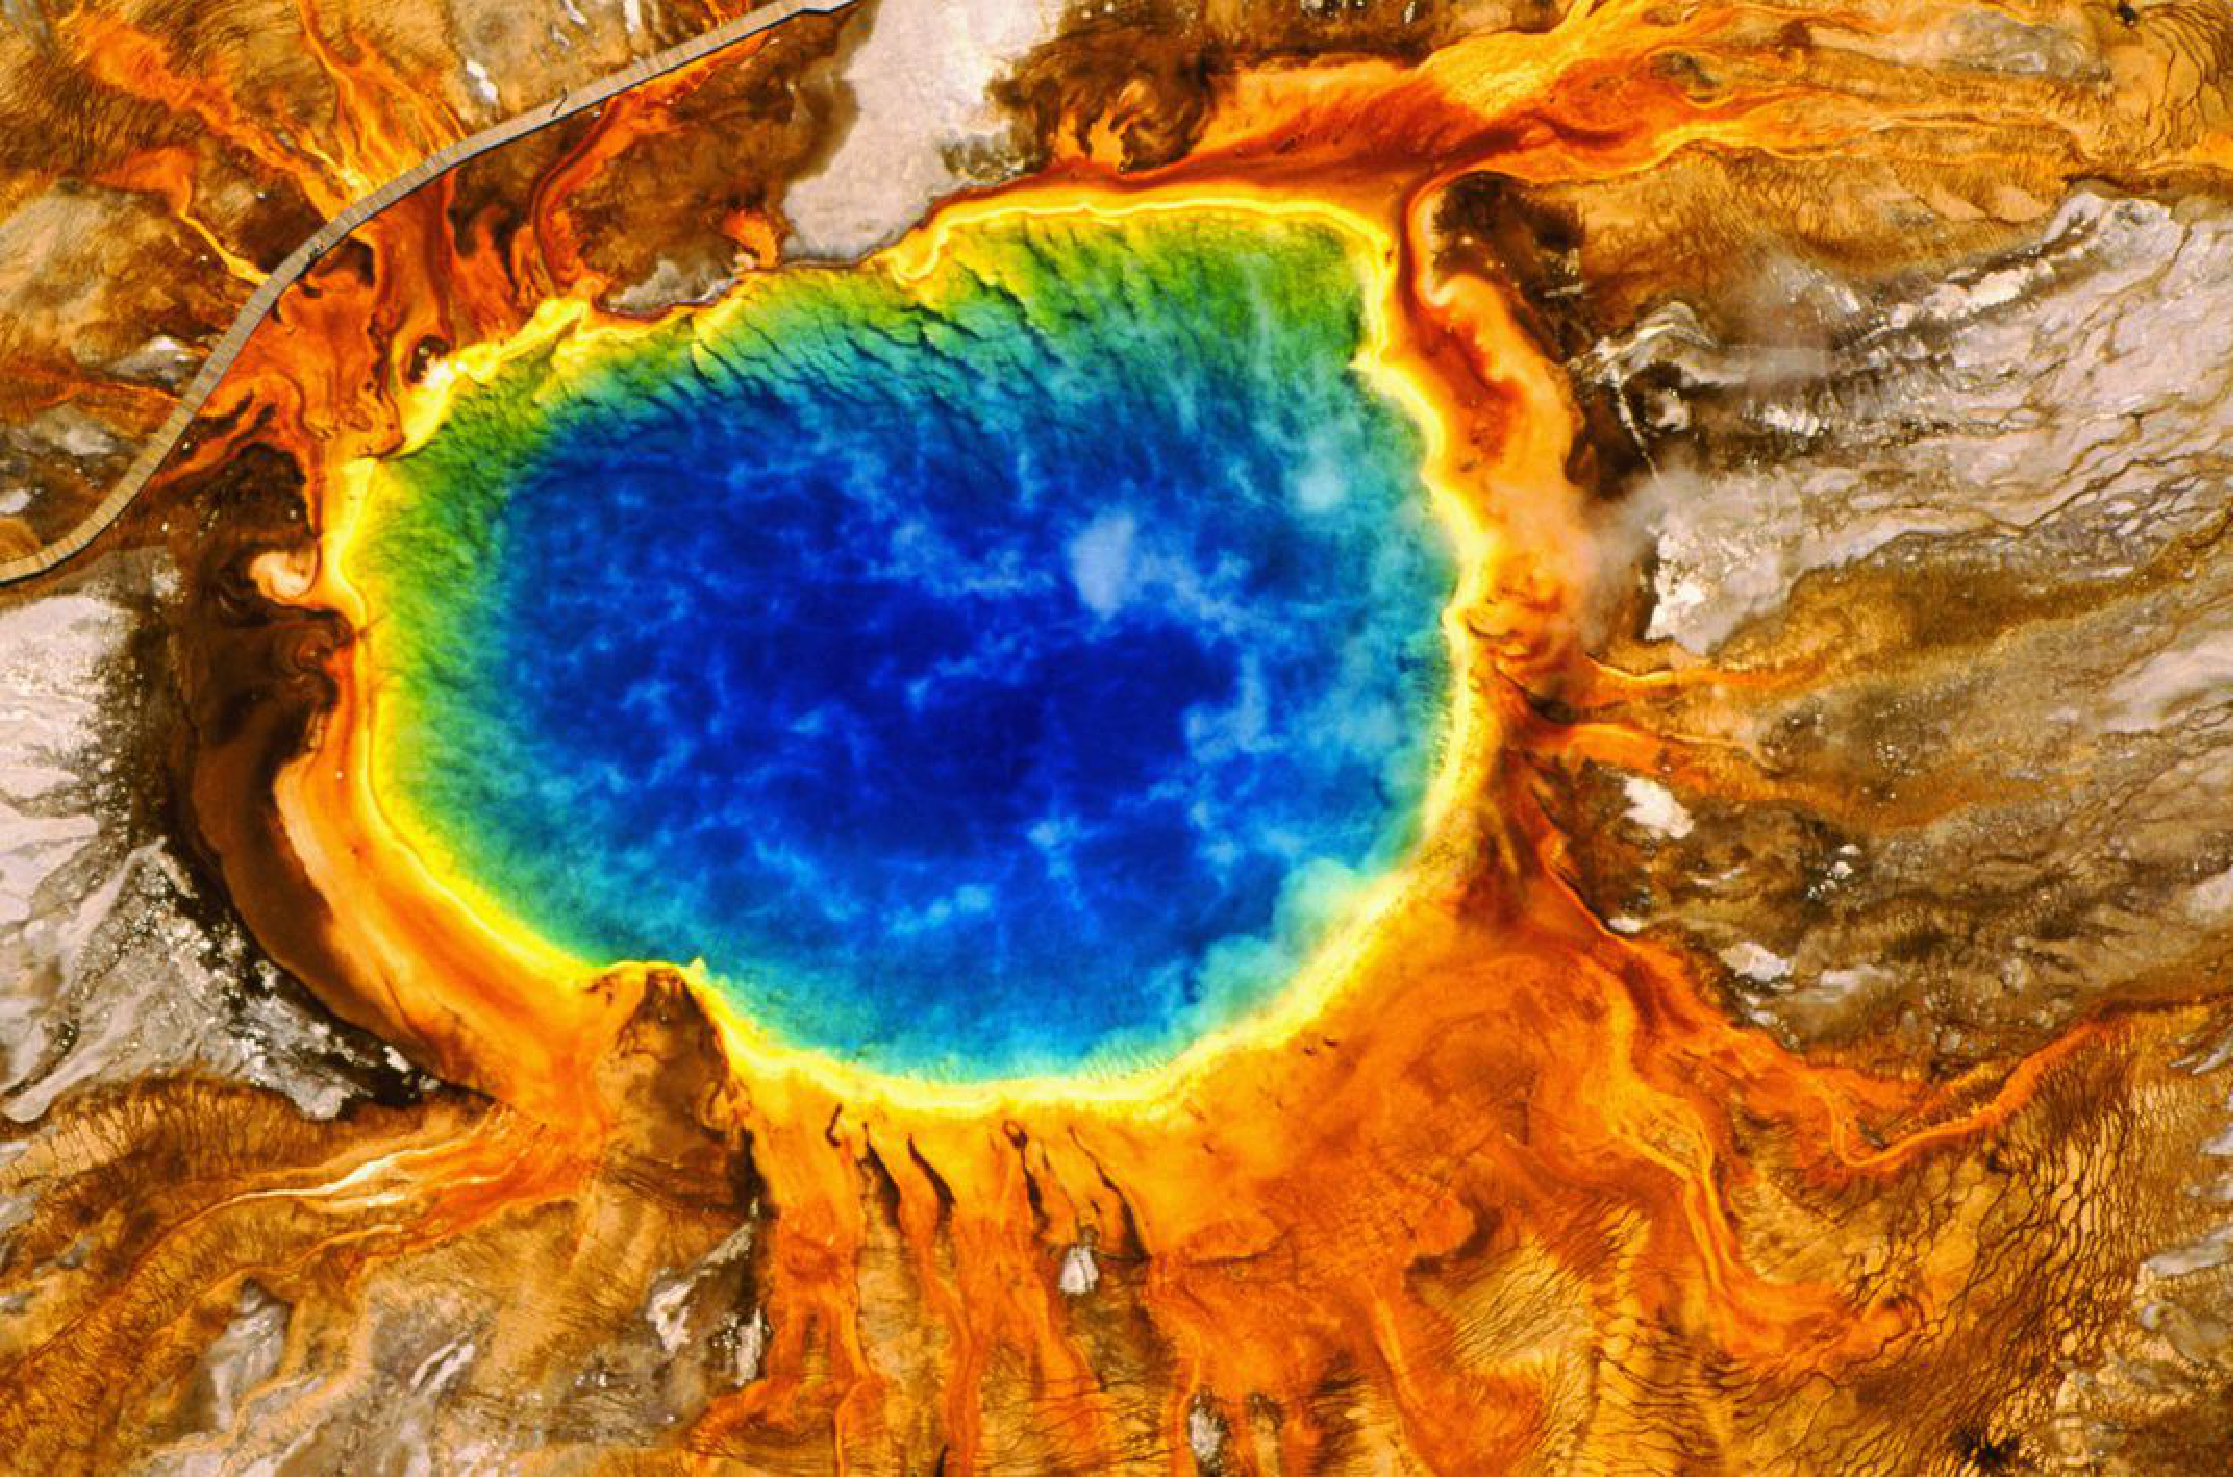
\includegraphics[height=0.5\columnwidth]{figures/applications/example-of-geochemical-reactions-in-yellowstone-geysers}
\caption*{Geochemical reaction calculations for thermal water analysis 
(Grand Prismatic, Midway Geyser Basin, Yellowstone, Wyoming, USA).}
\end{figure}
%
\end{singlespace}
%
\rcol
\begin{figure}
\vskip 5pt
\centering
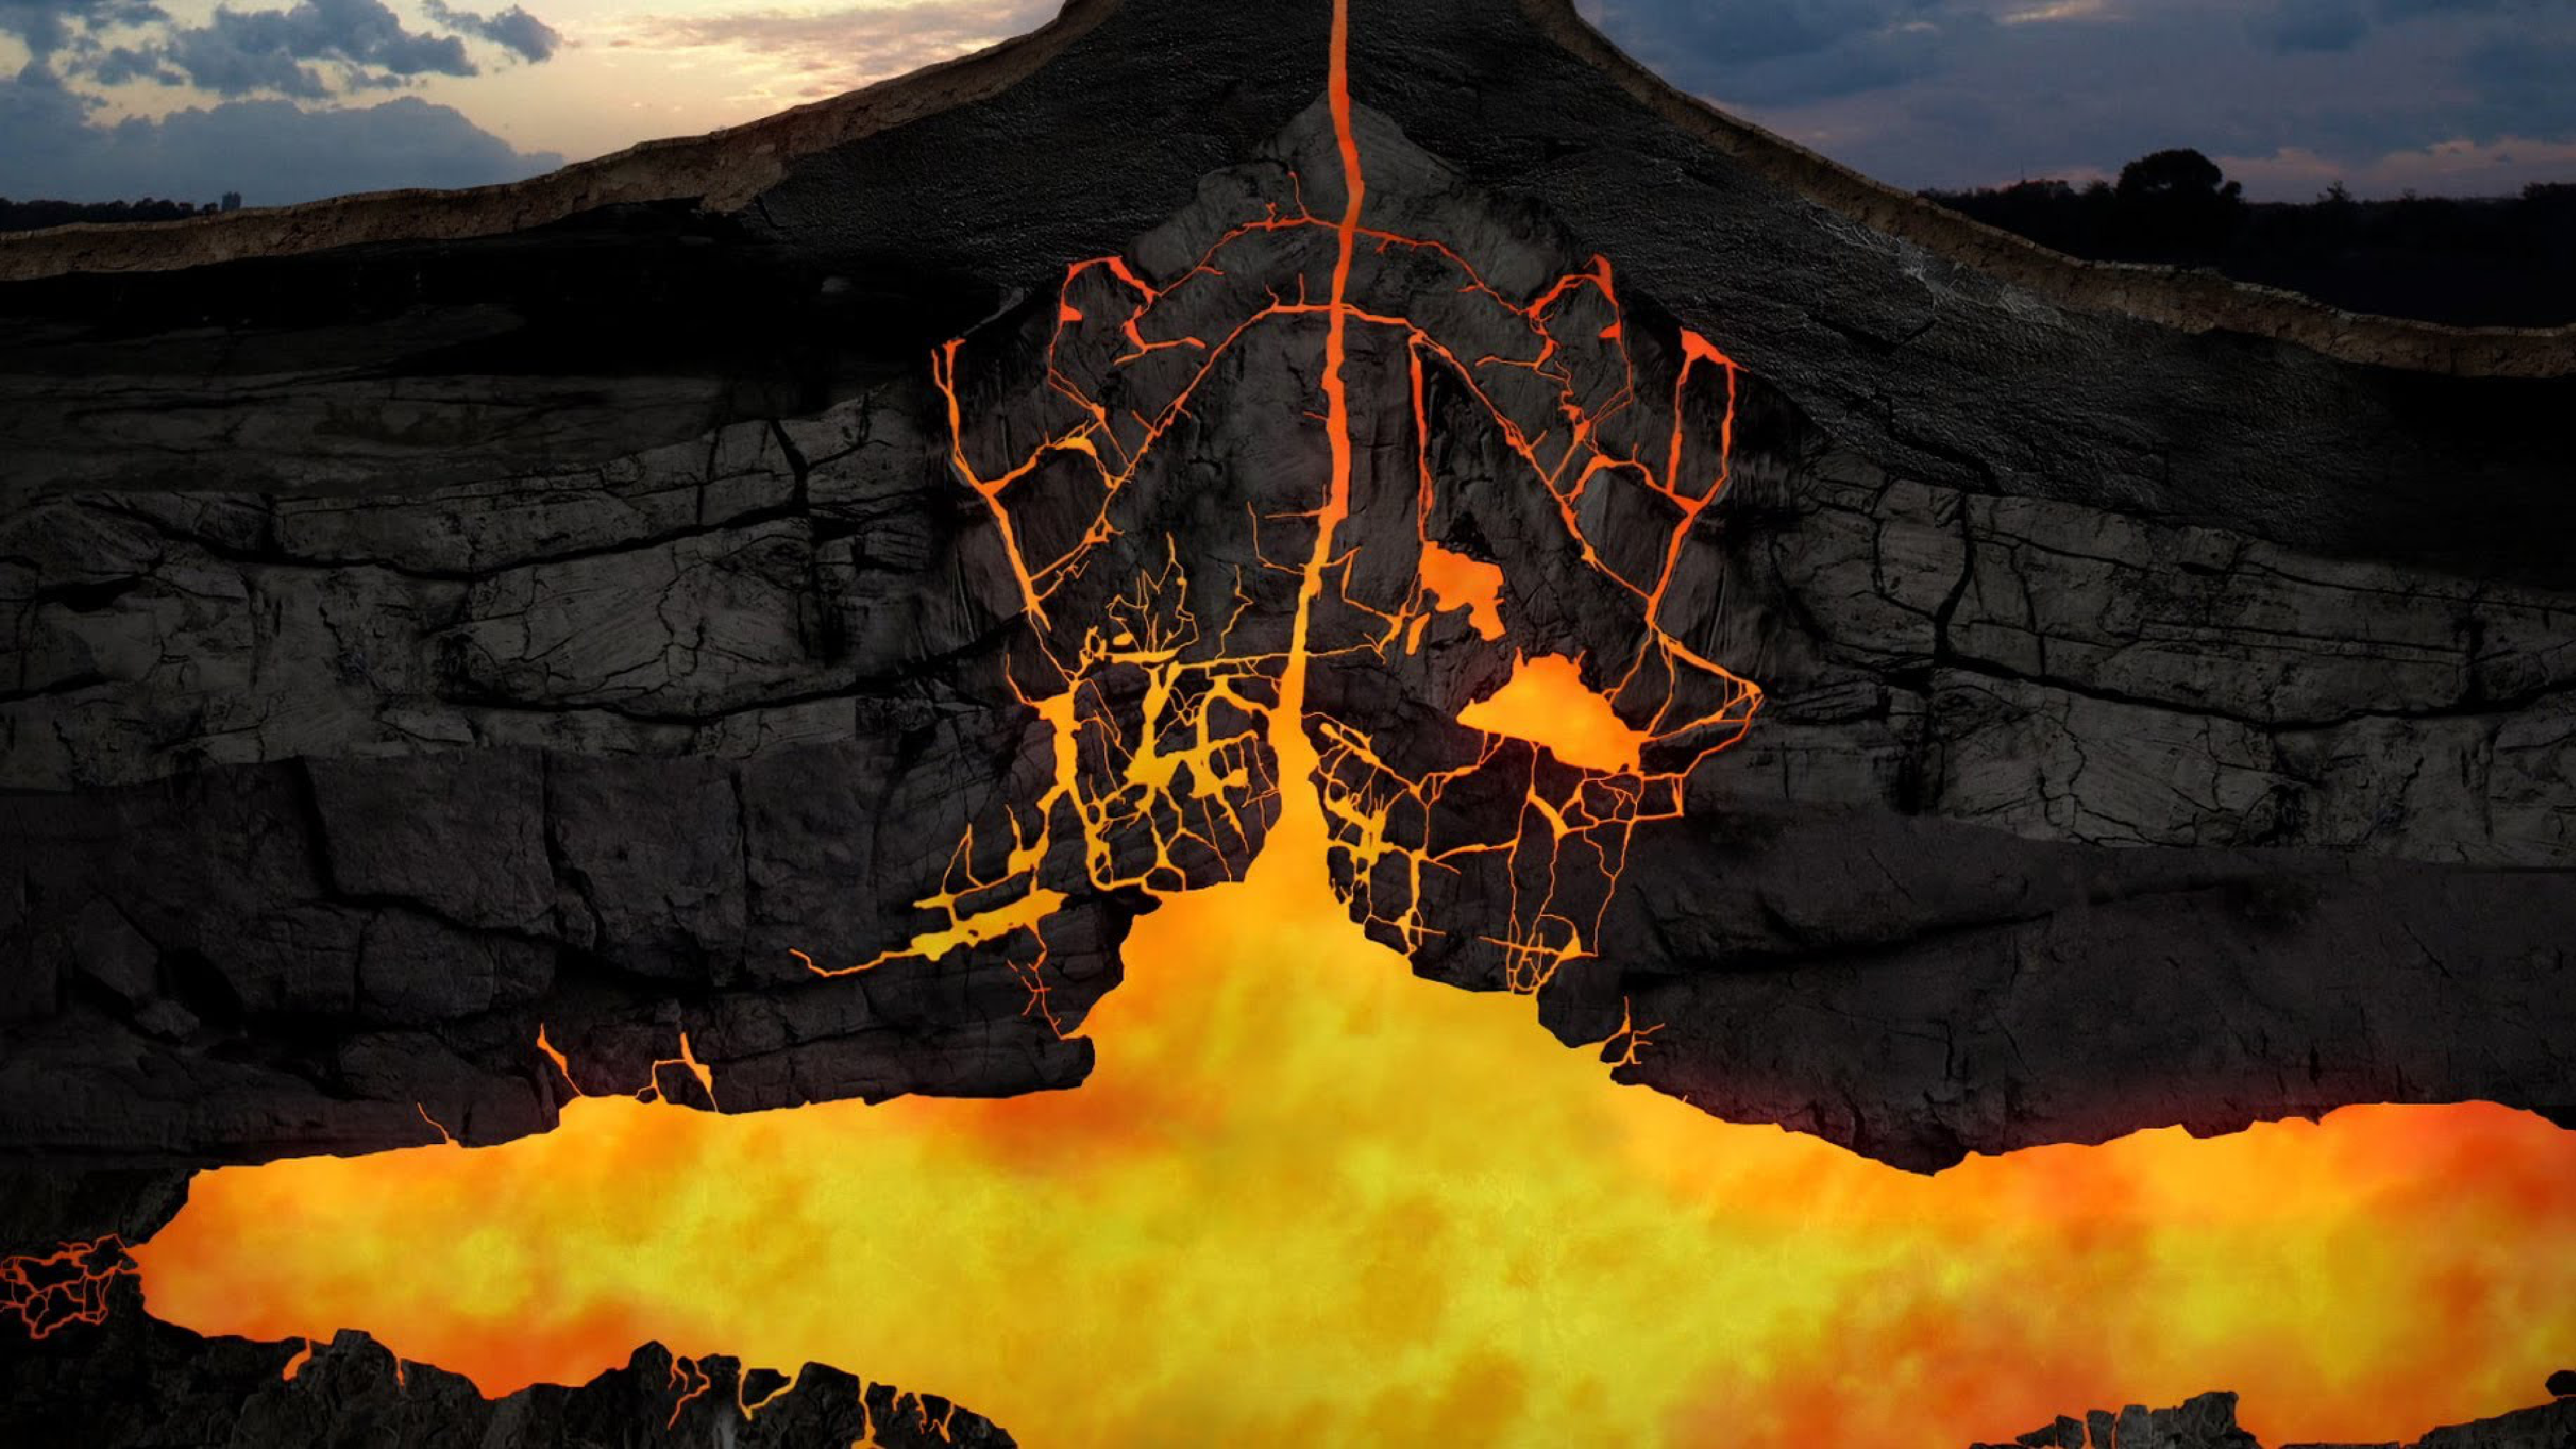
\includegraphics[height=0.5\columnwidth]{figures/applications/example-of-geochemical-reactions-in-a-volcano-magma-chamber}
\caption*{Geochemical reaction calculations for molten rocks as the magma flows
from the Earth's mantle upwards.}
\end{figure}
\ecol
\end{frame}

% --------------------------------------------------------------------------------------------------------------------%
% Geochemical modeling applications, Scaling prediction in wells
% --------------------------------------------------------------------------------------------------------------------%
%
\begin{frame}{Geochemical modeling applications, Scaling prediction in wells}
%
\lcol
%
\vskip 20pt
\begin{figure}
\centering
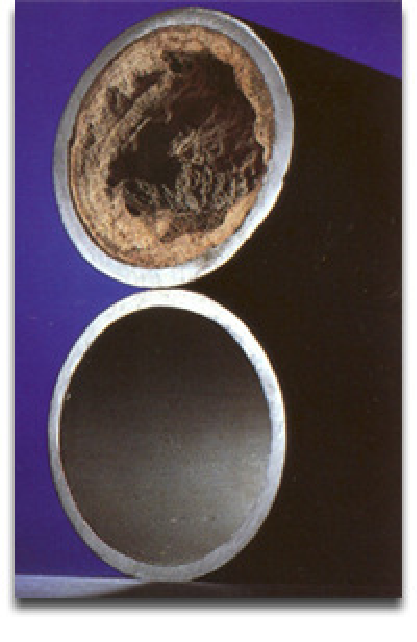
\includegraphics[height=0.6\textheight]{figures/applications/scaling-calcium-strontium-barium}
\caption*{Scale formation in a well as a result of geochemical reactions leading
to mineral precipitation.}
\end{figure}
%
\rcol
\vskip -20pt
\begin{itemize}[<+->]
\item Fluids coming from a reservoir experiences \textbf{temperature\slash pressure
changes along the wells}.
\item The decrease in temperature and/or pressure can lead to chemical reactions 
promoting precipitation of minerals and thus \textbf{scale formation} along the well.
\item Geochemical modeling can be used to \textbf{predict}, \textbf{understand},
and \textbf{assist }on the \textbf{\alert{\textbf{remediation of scale formation}}}.
\end{itemize}
\ecol
%
\end{frame}

% --------------------------------------------------------------------------------------------------------------------%
% Geochemical modeling applications: CO$_{\boldsymbol{2}}$ storage
% in geologic formations
% --------------------------------------------------------------------------------------------------------------------%
%
\begin{frame}{Geochemical modeling applications, 
CO$_{\boldsymbol{2}}$ storage in geologic formations}
%
\vskip 10pt
\lcol
%
\begin{figure}
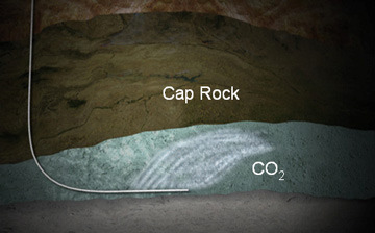
\includegraphics[height=3.8cm]{figures/applications/co2-storage-injection}
\caption*{Once CO$_{2}$ is injected in a deep saline aquifer, it starts to
\textbf{dissolve into the resident brine}. Geochemical calculations
can be used to calculate how much CO$_{2}$ dissolves and how much
CO$_{2}$ continues mobile as gas or supercritical fluid.}
\end{figure}
%
\rcol
%
\begin{figure}
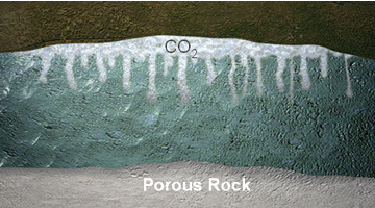
\includegraphics[height=3.8cm]{figures/applications/co2-storage-fingers}
\caption*{Brine with dissolved CO$_{2}$ becomes acidic. It can then more easily 
\textbf{react with rock minerals}. This change rock properties, such as \textbf{porosity} 
and \textbf{permeability}. Geochemical calculations can tell {\bf how much rock 
minerals dissolve}.}
\end{figure}
%
\ecol
%
\end{frame}
%
% --------------------------------------------------------------------------------------------------------------------%
% Geochemical modeling applications: Water analysis
% --------------------------------------------------------------------------------------------------------------------%
%
\begin{frame}{Geochemical modeling applications, Water analysis}
%
Given the following water analysis, with the concentration of many chemical elements and 
pH, \textbf{find the concentrations of all aqueous species in the water}:
\lcol
\begin{figure}
\centering
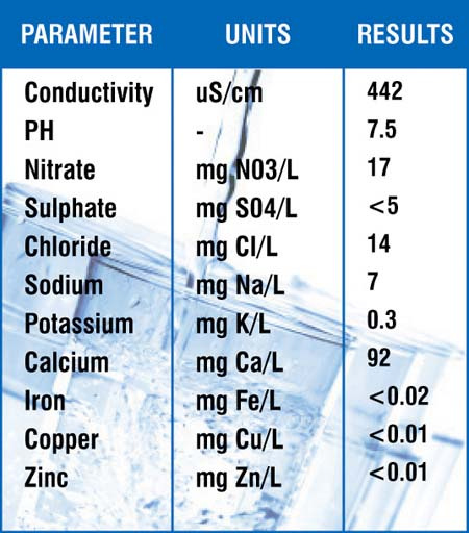
\includegraphics[height=0.6\textheight]{figures/applications/water-analysis}
\caption*{Water composition as a result of a water analysis.}
\end{figure}
\rcol
%
\begin{figure}
\centering
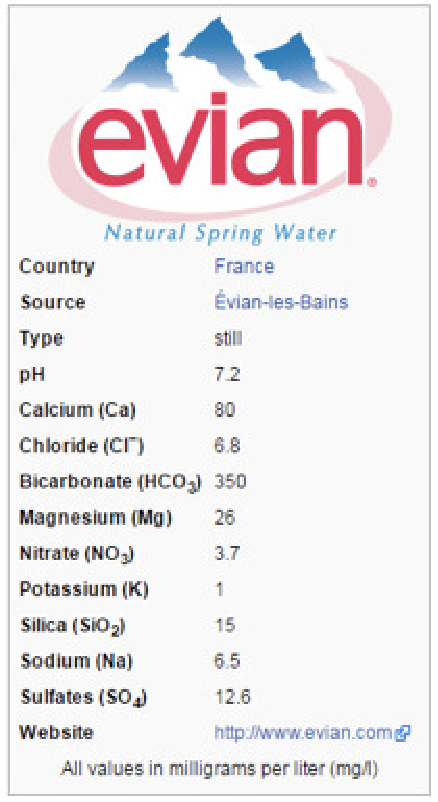
\includegraphics[height=0.6\textheight]{figures/applications/evian-chemical-water-composition}
\caption*{See Jupyter notebook tutorial \href{https://github.com/mtsveta/reaktoro-v2-workshop/blob/main/tutorials/applications/evian-water-analysis.ipynb}{\textcolor{indigo(dye)}{\it Analysis of the Evian water}}.}
\end{figure}
%
\ecol
%
\end{frame}

% --------------------------------------------------------------------------------------------------------------------%
% Geochemical modeling applications: Water analysis, Part II
% --------------------------------------------------------------------------------------------------------------------%
%
\begin{frame}{Geochemical modeling applications: Water analysis}
\textbf{Selected aqueous species} that could exist in that water sample:
\vskip 1pt
{\scriptsize%
\begin{tabular*}{1\columnwidth}{@{\extracolsep{\fill}}ccccccc}
Cl-(aq) & CuO(aq) & H2(aq) & HNO2(aq) & KSO4-(aq) & OH-(aq) & SO3-{}-(aq)
\tabularnewline
ClO-(aq) & CuO2-{}-(aq) & H2N2O2(aq) & HNO3(aq) & N2(aq) & S2-{}-(aq) & SO4-{}-(aq)\tabularnewline
ClO2-(aq) & CuOH+(aq) & H2O(aq) & HO2-(aq) & N2H5+(aq) & S2O3-{}-(aq) & Zn++(aq)\tabularnewline
ClO3-(aq) & Fe++(aq) & H2O2(aq) & HS-(aq) & N2H6++(aq) & S2O4-{}-(aq) & ZnCl+(aq)\tabularnewline
ClO4-(aq) & Fe+++(aq) & H2S(aq) & HS2O3-(aq) & N2O2-{}-(aq) & S2O5-{}-(aq) & ZnCl2(aq)\tabularnewline
Cu+(aq) & FeCl+(aq) & H2S2O3(aq) & HS2O4-(aq) & NH3(aq) & S2O6-{}-(aq) & ZnCl3-(aq)\tabularnewline
Cu++(aq) & FeCl++(aq) & H2S2O4(aq) & HSO3-(aq) & NH4+(aq) & S2O8-{}-(aq) & ZnO(aq)\tabularnewline
CuCl(aq) & FeCl2(aq) & HCl(aq) & HSO4-(aq) & NO2-(aq) & S3-{}-(aq) & ZnO2-{}-(aq)\tabularnewline
CuCl+(aq) & FeO(aq) & HClO(aq) & HSO5-(aq) & NO3-(aq) & S3O6-{}-(aq) & ZnOH+(aq)\tabularnewline
CuCl2(aq) & FeO+(aq) & HClO2(aq) & HZnO2-(aq) & Na+(aq) & S4-{}-(aq) & \tabularnewline
CuCl2-(aq) & FeO2-(aq) & HCuO2-(aq) & K+(aq) & NaCl(aq) & S4O6-{}-(aq) & \tabularnewline
CuCl3-(aq) & FeOH+(aq) & HFeO2(aq) & KCl(aq) & NaOH(aq) & S5-{}-(aq) & \tabularnewline
CuCl3-{}-(aq) & FeOH++(aq) & HFeO2-(aq) & KHSO4(aq) & NaSO4-(aq) & S5O6-{}-(aq) & \tabularnewline
CuCl4-{}-(aq) & H+(aq) & HN2O2-(aq) & KOH(aq) & O2(aq) & SO2(aq) & \tabularnewline
\end{tabular*}}

\pause
\vskip 5pt
\alert{\textbf{Questions}} we want to answer: 
\begin{itemize}
\item What are the \textbf{amounts of these species}? 
\item How \textbf{saturated} is the water \textbf{with respect to several minerals}? \\
\textbf{Note:}  \emph{saturation} is the tendency of the solution to dissolve/precipitate a mineral.
\end{itemize}
\end{frame}
%
% --------------------------------------------------------------------------------------------------------------------%
% Other applications for geochemical modeling
% --------------------------------------------------------------------------------------------------------------------%
%
\begin{frame}{Other applications for geochemical modeling}
\begin{itemize}
\item Geochemical reaction calculations can be used for a wide range of
\textbf{industrial and environmental applications}: 
\begin{itemize}
\item nuclear waste management to ensure radionuclides remain properly stored
for thousands\slash millions of years;
\item ore-forming processes;
\item geochemical reactions in geothermal and hydrothermal systems;
\item enhanced oil and gas recovery (prediction of gas and mineral solubility 
at the wide range of temperatures and pressures);
\item transport of reactive solution in porous and fractured media.
\end{itemize}
\end{itemize}

\begin{figure}
\centering
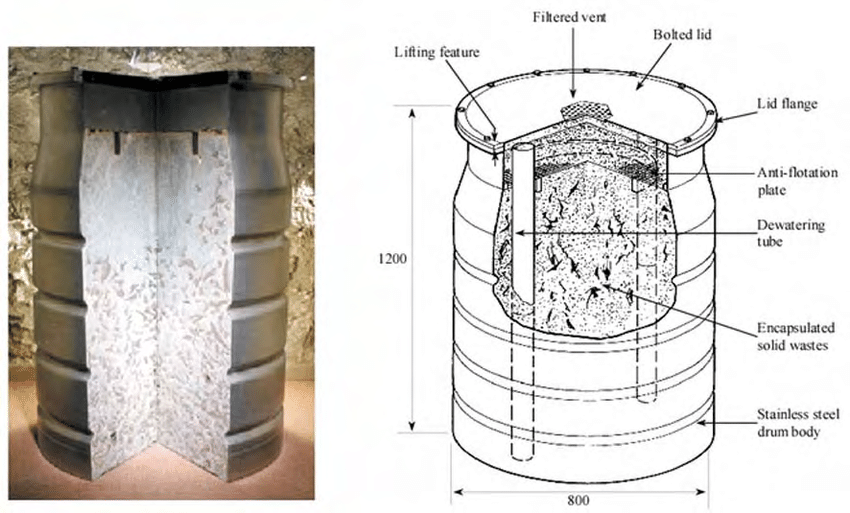
\includegraphics[height=0.2\columnwidth]{figures/applications/waste-storage.png} \quad %\caption*{Radioactive waste captured in cement.}
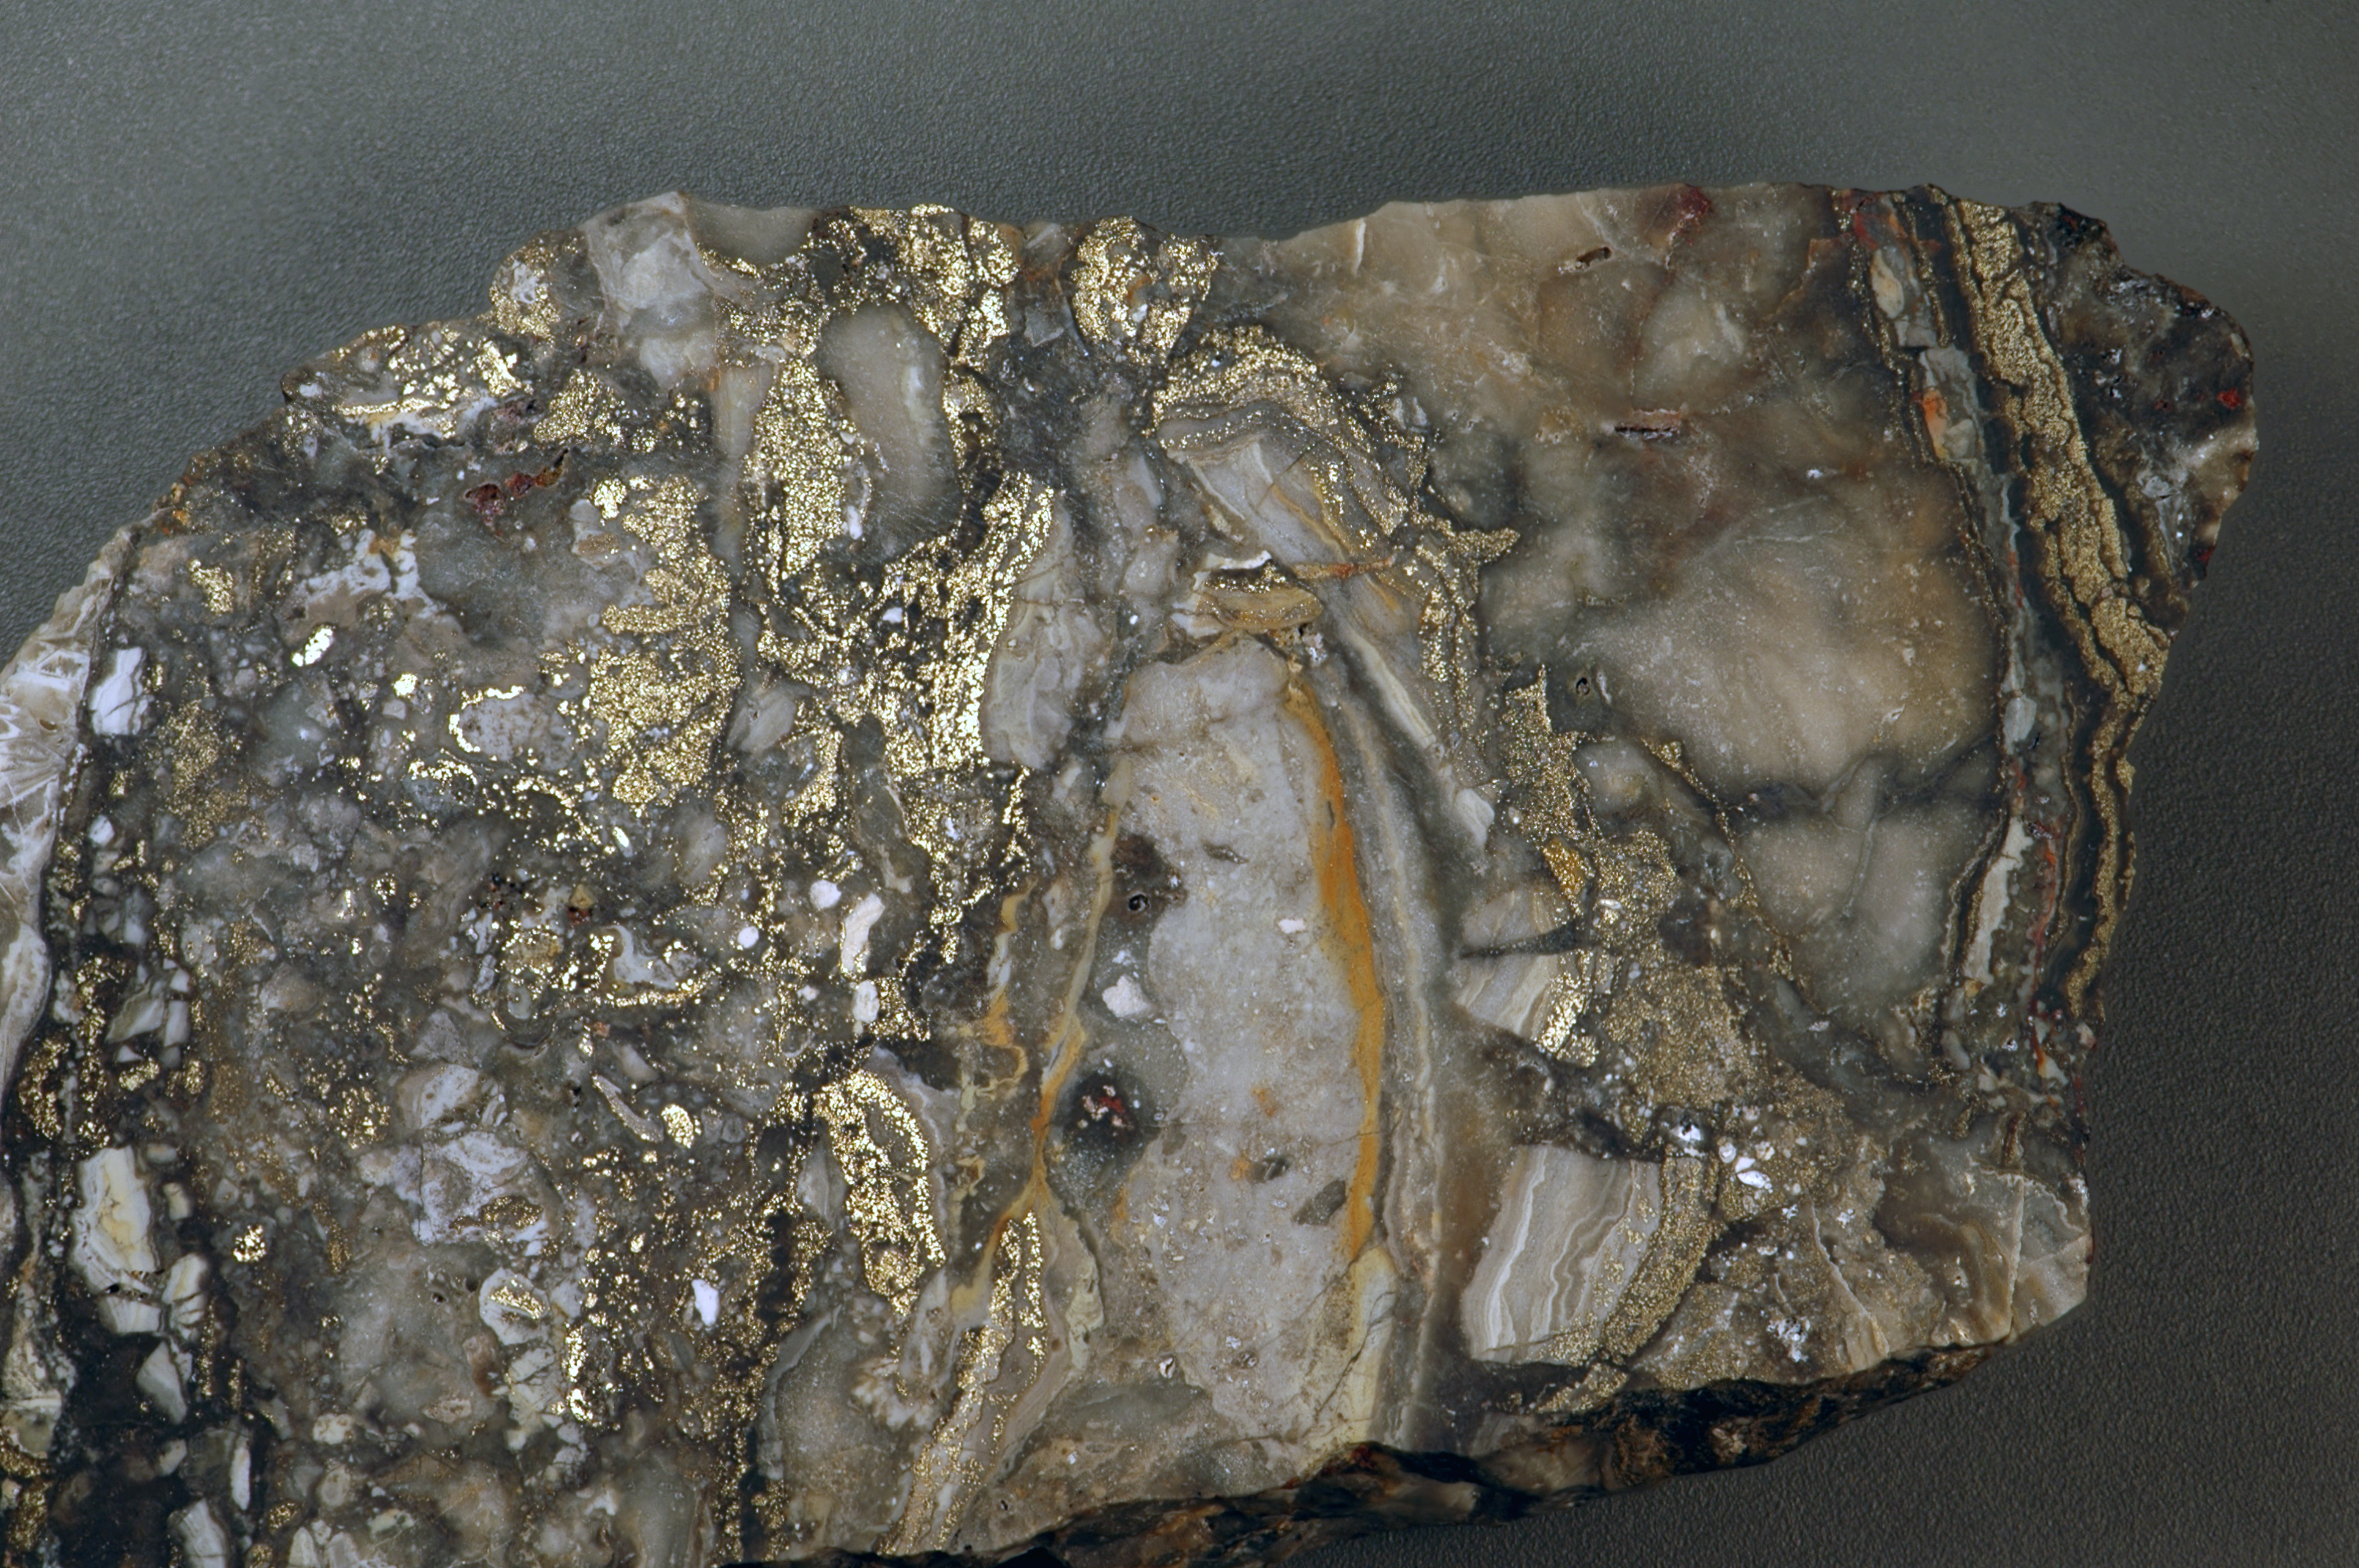
\includegraphics[height=0.2\columnwidth]{figures/applications/ore-forming.jpg}  \quad %\caption*{Ore forming processes.}
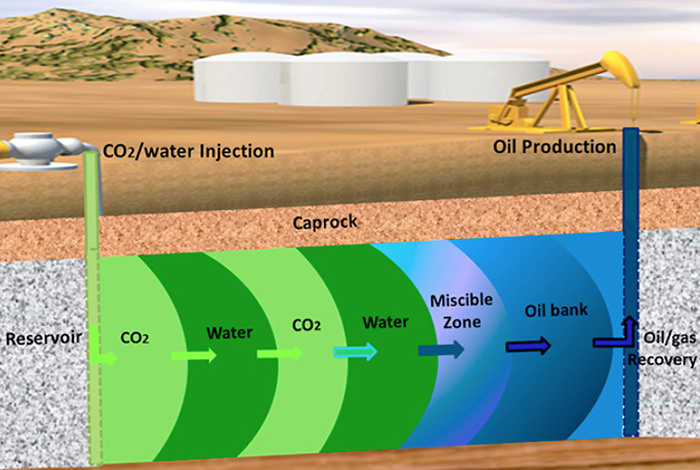
\includegraphics[height=0.2\columnwidth]{figures/applications/enhanced-oil-recovery.jpg}%\caption*{Enhanced oil and gas recovery.}
\end{figure}

\end{frame}

\subsection{Chemical equilibrium and chemical kinetics for modeling geochemical
systems}

% --------------------------------------------------------------------------------------------------------------------%
% Intuition about chemical reaction behavior
% --------------------------------------------------------------------------------------------------------------------%

\begin{frame}{Chemical reaction behavior,  Initial intuition}
	\vskip 5pt
\begin{itemize}
\item Consider 1 kg of H$_{2}$O mixed with 1 mg of NaCl (halite). 
\pause
\item Chemical reactions that occur among the species in the solution and the halite are as follows:\\[-30pt]
\begin{align*}
\mathsf{NaCl(halite, s)} & \rightleftharpoons\mathsf{Na^{+}+Cl^{-}}\\
\mathsf{Na^{+}+Cl^{-}} & \rightleftharpoons\mathsf{NaCl(aq)}\\
\mathsf{H_{2}O} & \rightleftharpoons\mathsf{H^{+}+OH^{-}}
\end{align*}
\vskip -5pt
\pause
\item Detailed steps: 
\begin{itemize}
\item \textbf{pure water} solution contains species: H$_2$O, H$^+$, OH$^-$, O$_2$(aq), H$_2$(aq)
\item \textbf{scale of the species} in water solution: 
55.508 mol of H$_2$O, 1e-7 mol of H$^+$, 1e-7 mol of OH$^-$ (to make sure the charge balance),
 1e-31 mol of O$_2$(aq),  1e-31 mol of H$_2$(aq) 
\item after \textbf{mixing} NaCl(s) we have in addition: Na$^{+}$, Cl$^{-}$, NaCl(aq), HCl(aq), NaOH(aq)
\item  \textbf{new ions} H$^+$ and Cl$^{-}$ produce $\mathsf{H^{+}+Cl^{-}} \rightleftharpoons \mathsf{HCl(aq)}$
\end{itemize}
\pause
\item What can we say about the \alert{\textbf{behavior and time-scale}} of the these species after 1 ms, 1 s, 1 min?
\end{itemize}
\end{frame}

\begin{frame}{Poll on chemical equilibrium and kinetics }
\alert{\bf Quiz}: In a context of this example and kinetic/equilibrium simulations, make a guess on which statement is correct?
\begin{center}
\vskip 10pt
{\Large \href{http://etc.ch/M2Rp}{\textcolor{indigo(dye)}{\tt http://etc.ch/M2Rp}}}
or 

\includegraphics[height=0.25\columnwidth]{figures/intro/poll.png}
\end{center}    
%
% \hiddenpause
% {\bf Answer}: \\
% \qquad $\bullet$ The chemical processes of the time scale of 1 ms are governed by equilibrium. \\ 
% \qquad $\bullet$ The chemical processes of the time scale of 1 min are governed by kinetics.
\end{frame}
%
% --------------------------------------------------------------------------------------------------------------------%
% Chemical kinetics vs. chemical equilibrium
% --------------------------------------------------------------------------------------------------------------------%

\begin{frame}{Chemical kinetics vs. Chemical equilibrium}
%
\small
\lcol
\vskip 10pt
\begin{cbox}{Chemical Kinetics}
$\bullet$ Focuses on \alert{\textbf{pathways of reactions}} and  \alert{\textbf{their rate}}. \\
$\bullet$ Used to compute the amounts of the reacting species \alert{\textbf{over time}}. \\
\end{cbox}

\begin{cbox}{Chemical Equilibrium} 
$\bullet$ Focuses on the reactions with \alert{\textbf{no changes in the amount of reactants and products}}. \\
$\bullet$ Used to directly compute the final composition of the species when
the reactions are \alert{\textbf{in equilibrium}}. 
\end{cbox}

\rcol

\vskip 10pt
\begin{figure}
\centering
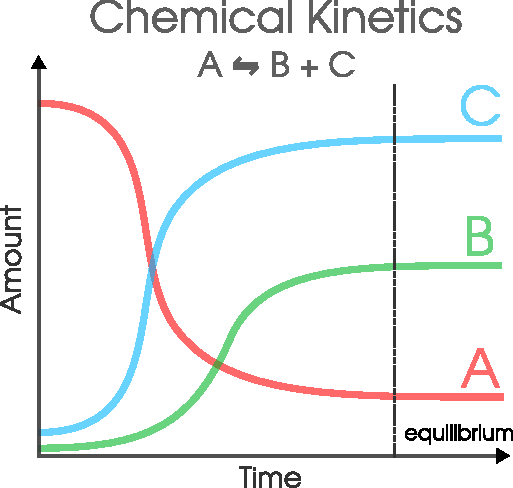
\includegraphics[width=0.8\columnwidth]{figures/applications/chemical-kinetics-equilibrium-illustration-evolution-plot}
\caption*{Chemical kinetics evolution of species A, B, and C over time.}
\end{figure}

\ecol

\end{frame}

% --------------------------------------------------------------------------------------------------------------------%
% Examples of chemical equilibrium reactions
% --------------------------------------------------------------------------------------------------------------------%

\begin{frame}{Examples of chemical equilibrium reactions}
%
\lcol

\begin{itemize}
	\item \alert{\textbf{Bottle with soda drink}}
	\begin{itemize}
		\item CO$_2$(g) dissolved in the liquid
		\item CO$_2$(g) is in the space between the liquid and the cap
		\item CO$_2$ is constantly moving from the liquid to the gas phase, and back
		\begin{align*}
			\mathsf{CO_2(g) + H2O(l)} & \rightleftharpoons \mathsf{H_2CO_3(aq)}
		\end{align*}
	\end{itemize}
%
	\pause
	\item \alert{\textbf{(Oxy)haemoglobin reactions in blood}}
	\begin{itemize}
		\item haemoglobin takes up oxygen and releases it
		\begin{align*}
			\mathsf{haemoglobin(aq) + 4 O_2(g) } & \rightleftharpoons 	
			\mathsf{haemoglobin(O_2)_4(aq)}
		\end{align*}
		\item oxyhaemoglobin goes through the blood stream to cells
	\end{itemize}
\end{itemize}      

\rcol

\begin{figure}
\centering
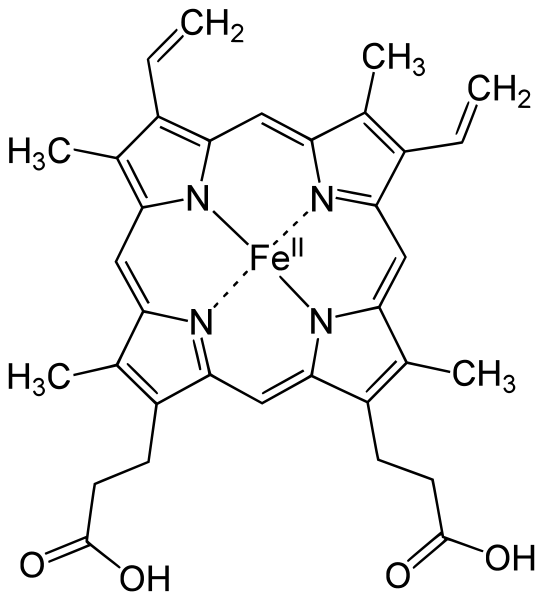
\includegraphics[width=0.8\columnwidth]{figures/applications/hemoglobin.png}
\caption*{Hemoglobin structure.}
\end{figure}

\ecol

\end{frame}

% --------------------------------------------------------------------------------------------------------------------%
% Examples of chemical kinetics reactions
% --------------------------------------------------------------------------------------------------------------------%

\begin{frame}{Examples of chemical kinetics reactions}
%
\lcol

\begin{itemize}
	\item \alert{\textbf{Corrosion}}, a natural process that converts a refined metal into a more chemically stable form such as oxide, hydroxide, or sulfide.
		\begin{itemize}
		\item galvanic corrosion 
		\item electrolytic corrosion
		\item microbial corrosion
		\item high temperature corrosion
	\end{itemize}
	%
	\pause
	\item \alert{\textbf{Fluid catalytic cracking (FCC)}}, a conversion process of petroleum crude oils into gasoline, olefinic gases, and other products. Used in petroleum refineries.
\end{itemize}      

\rcol

\begin{figure}
\centering
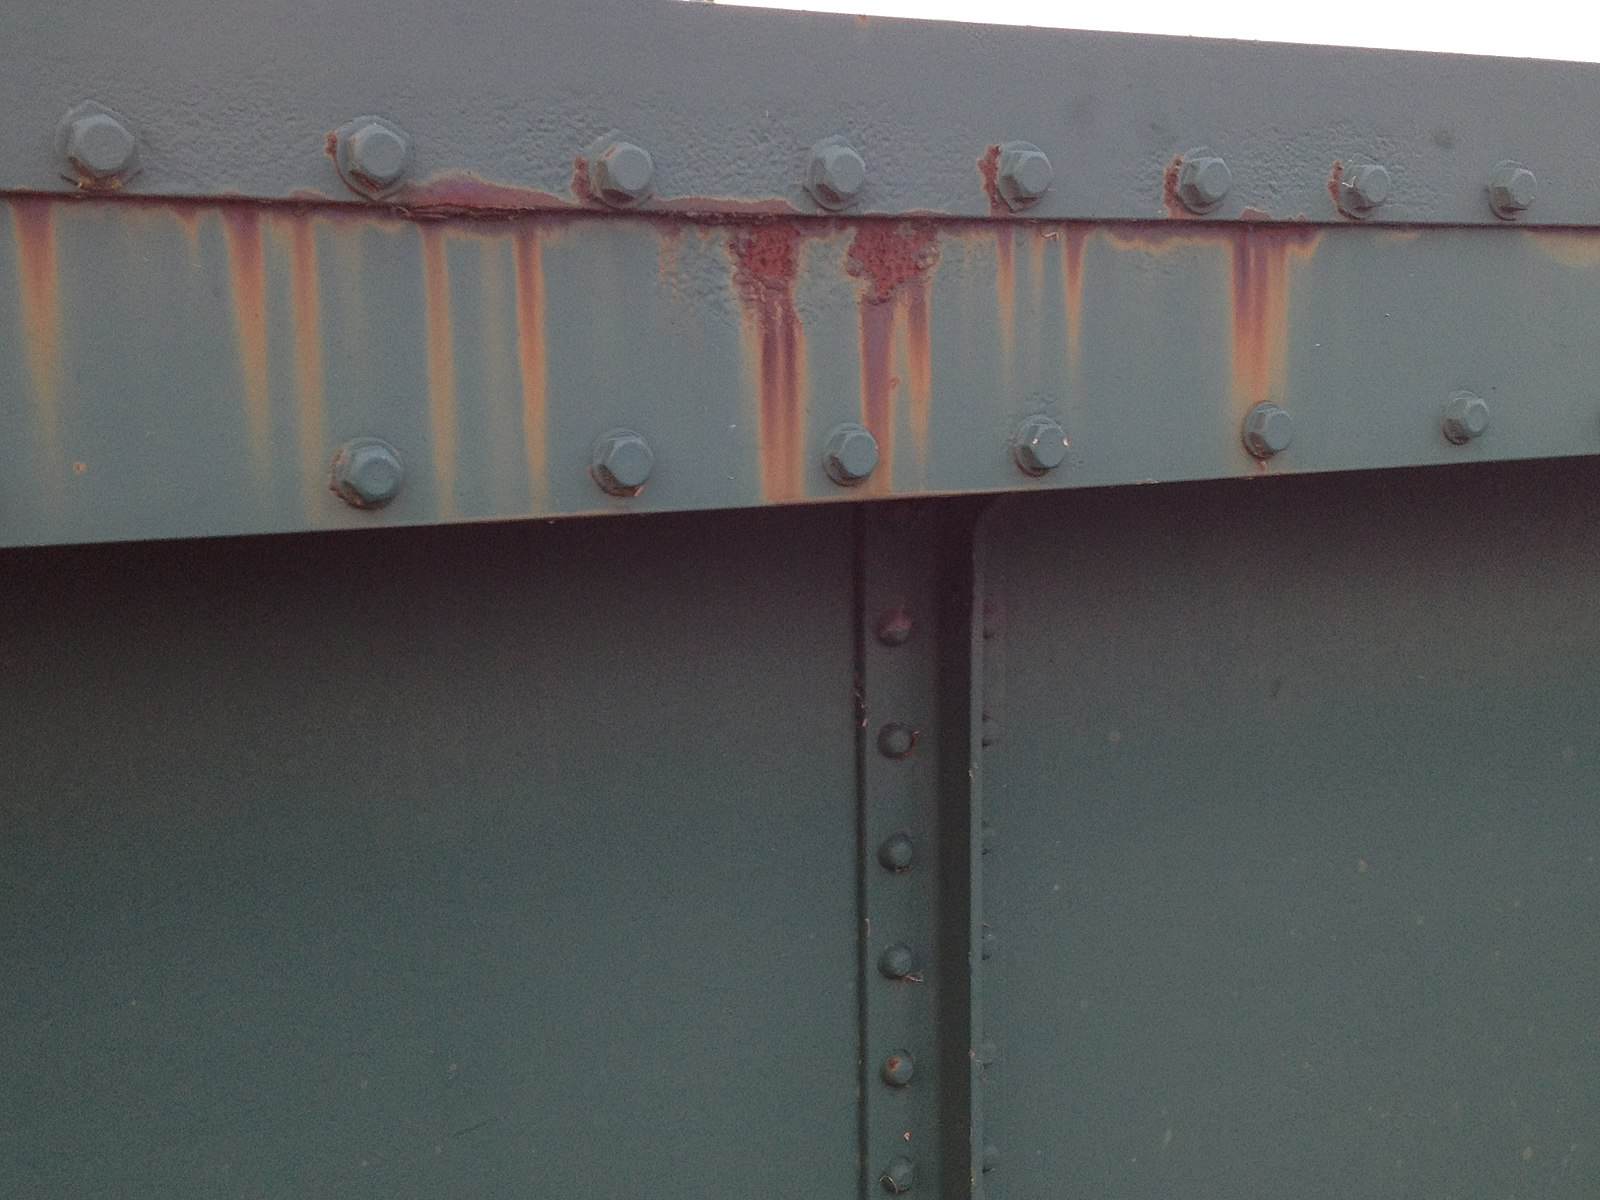
\includegraphics[width=0.45\columnwidth]{figures/applications/corrosion.jpg} \\[5pt]
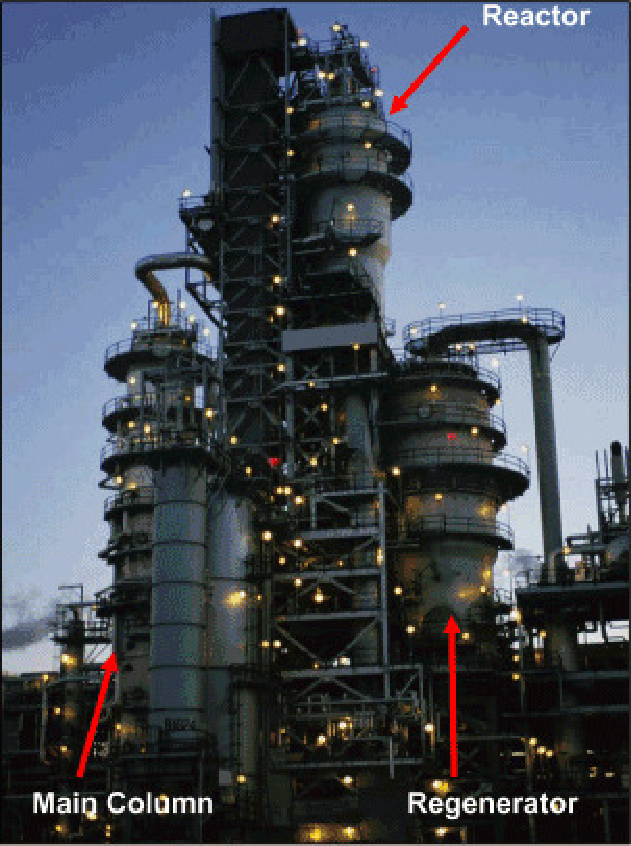
\includegraphics[width=0.45\columnwidth]{figures/applications/fluid-catalytic-cracker}
%\caption*{Hemoglobin structure.}
\end{figure}

\ecol

\end{frame}
%
% --------------------------------------------------------------------------------------------------------------------%
% Chemical equilibrium, Practical observations
% --------------------------------------------------------------------------------------------------------------------%
%
\subsection{Practical observations on chemical equilibrium}
%
% --------------------------------------------------------------------------------------------------------------------%
% Reaction classification
% --------------------------------------------------------------------------------------------------------------------%
%
\begin{frame}{Reaction classification}
	\begin{itemize}
		\item \alert{\bf Irreversible} or \alert{\bf reversible}:
		\begin{itemize}
			\item An {\bf irreversible} reaction is one that occurs in only one direction and continues in this direction until at least one of the reactants is depleted.
			\item A {\bf reversible} reaction can occur in both directions (with forward and backward reaction reaction coefficients $k_f$ and $k_b$, respectively):
			%
			\[	
			\mathsf{a\,A + b\,B} \xrightleftharpoons[k_b]{k_f} \mathsf{c\,C + d\,D}.
			%\quad 
			%\mbox{with equilibrium constant}
			\quad
			%K_e := \tfrac{k_f}{k_b} = \tfrac{\mathsf{[C]^c\, [D]^d}}{\mathsf{[A]^a\,[B]^b}}.
			\]
			%
		\end{itemize}
		%%%
		\item \alert{\bf Homogeneous} or \alert{\bf heterogeneous}:
		\begin{itemize}
			\item A {\bf homogeneous} reaction involves a single phase, e.g., 
			%
			\begin{alignat*}{2}
				\mbox{Formation of ammonia}:  \mathsf{N_2(g) + 3\,H_2(g) } & \mathsf{\xrightleftharpoons[]{} 2\,NH_3(g)}\\
				\mbox{Oxidation of sulfur dioxide}: \mathsf{2\,SO_2(g) + O_2(g) } & \mathsf{\xrightleftharpoons[]{} 2\,SO_3(g)} 
			\end{alignat*}
			%
			\item A {\bf heterogeneous} reaction involves more than one phase, e.g., 
			\begin{alignat*}{2}
				\mbox{Carbonation} : \mathsf{Ca(OH)_2(s) + CO_2(g)} & \mathsf{\xrightleftharpoons[]{} CaCO_3(s) + H_2O(l)}
			\end{alignat*}
		\end{itemize}
		
	\end{itemize}
\end{frame}
%
\begin{frame}{Practical observations on chemical equilibrium}
\vskip 10pt
\begin{itemize}
\item Chemical reactions \textbf{alter the amounts of species over time}, where species can be distributed among one or more phases (minerals, gaseous, mineral).
\pause
\item Each of these reactions have \textbf{forward and backward rates}. 
\pause
\item Consider the reaction
\[
\mathsf{A+B \xrightleftharpoons[k_b]{k_f} C+2\,D,}
\]
\pause
\item Rate of the reaction is measured in mol/s.
\pause
\item Assume at some time $t$ this reaction has a \textbf{forward rate}
of \alert{\textbf{2 mol/s}} and a \textbf{backward rate}
of \alert{\textbf{1 mol/s}}.
\pause
\item \alert{\textbf{Net rate of the reaction}} = \textbf{forward rate} - \textbf{backward rate}. 
\pause 
\item 
\textbf{forward rate} = \textbf{production rate} $>$ 0, \\
\textbf{backward rate} = \textbf{consumption rate} $<$ 0.
\end{itemize}
\end{frame}

\begin{frame}{Production and consumption rates}
	\vskip 10pt
Consider the reaction
	\[
	\mathsf{A+B\xrightleftharpoons[k_b]{k_f} C+2\,D.}
	\]
%
\alert{\textbf{Quiz:}} What is \textbf{rate of production\slash consumption}
of A, B, C and D (in mol/s)? \\
\begin{center}{ \href{http://etc.ch/M2Rp}{\textcolor{indigo(dye)}{\tt http://etc.ch/M2Rp}}} \quad
or \quad

\includegraphics[height=0.23\columnwidth]{figures/intro/poll.png}
\end{center}
% \hiddenpause
% \textbf{Answer:} \\
% \qquad $\bullet$ production rates are 1 mol/s for C, 2 mol/s for D; \\
% \qquad $\bullet$ consumption rates are -1 mol/s for A, -1 mol/s for B. 
\end{frame}
% --------------------------------------------------------------------------------------------------------------------%
% Chemical equilibrium of species
% --------------------------------------------------------------------------------------------------------------------%
%
\begin{frame}{Chemical equilibrium of species}
%
\alert{\textbf{Quiz:}} What happens when this \textbf{net rate} is \alert{\textbf{zero}} in a context of reaction 
%
\[
\mathsf{A+B \xrightleftharpoons[k_b]{k_f} C+2\,D?}
\]
%
\begin{center}{ \href{http://etc.ch/M2Rp}{\textcolor{indigo(dye)}{\tt http://etc.ch/M2Rp}}} \quad
or \quad

\includegraphics[height=0.23\columnwidth]{figures/intro/poll.png}
\end{center}
% \hiddenpause
% \textbf{Answer:} \\ 
% \qquad $\bullet$ the amounts of each species in the system \textbf{no longer experience any change}, and \\ 
% \qquad $\bullet$ they are in \alert{\textbf{chemical equilibrium}}.
% %
% \pause
% \alert{\textbf{Example:}}
% mixing 1 kg of H$_{2}$O with NaCl (halite):\\[-20pt] 
% %
% \begin{align*}
% \mathsf{NaCl(halite, s)} & \rightleftharpoons\mathsf{Na^{+}+Cl^{-}}\\[-1pt]
% \mathsf{Na^{+}+Cl^{-}} & \rightleftharpoons\mathsf{NaCl(aq)}\\[-1pt]
% \mathsf{H_{2}O} & \rightleftharpoons\mathsf{H^{+}+OH^{-}}
% \end{align*}
% %
% \vskip -5pt
% \pause
% \begin{itemize}
% %
% \item If we take \alert{\textbf{1 mg of NaCl}}, eventually, all salt fully dissolves, so the net rate of production of Na$^{+}$ and C$^-$ becomes zero.
% %%\item we have reached the \textbf{chemical equilibrium} of the system. 
% %\end{itemize}
% %
% \pause
% \item If we take \alert{\textbf{100 mg of NaCl }}: eventually, water solution will be saturated with the salt, so Na$^{+}$ and C$^-$  is precipitating NaCl with the similar rate as it is dissolving.
% %%\item we have reached the \textbf{chemical equilibrium} of the system. 
% %\end{itemize}
% \end{itemize}
% \pause
% \alert{\textbf{Note}}: See a Jupyter notebook \href{https://github.com/mtsveta/reaktoro-v2-workshop/blob/main/tutorials/solubility/solubility-tablesalt-water.ipynb}{\textcolor{indigo(dye)}{\it On mixing table salt with water}}.

\end{frame}
%
\begin{frame}{Example explaining the reaction net rate}
%
Let us mix 1 kg of H$_{2}$O with NaCl (halite):\\[-20pt] 
%
\begin{align*}
\mathsf{NaCl(halite, s)} & \rightleftharpoons\mathsf{Na^{+}+Cl^{-}}\\[-1pt]
\mathsf{Na^{+}+Cl^{-}} & \rightleftharpoons\mathsf{NaCl(aq)}\\[-1pt]
\mathsf{H_{2}O} & \rightleftharpoons\mathsf{H^{+}+OH^{-}}
\end{align*}
%
\vskip -5pt
\pause
Let us consider \textbf{two scenarios}:
\begin{itemize}
%
\item If we take \alert{\textbf{1 mg of NaCl}}, eventually, all salt fully dissolves, so the net rate of production of Na$^{+}$ and C$^-$ becomes zero.
%%\item we have reached the \textbf{chemical equilibrium} of the system. 
%\end{itemize}
%
\pause
\item If we take \alert{\textbf{100 mg of NaCl }}: eventually, water solution will be saturated with the salt, so Na$^{+}$ and C$^-$  is precipitating NaCl with the similar rate as it is dissolving.
%%\item we have reached the \textbf{chemical equilibrium} of the system. 
%\end{itemize}
\end{itemize}
\pause
\alert{\textbf{Note}}: See a Jupyter notebook \href{https://github.com/mtsveta/reaktoro-v2-workshop/blob/main/tutorials/solubility/solubility-tablesalt-water.ipynb}{\textcolor{indigo(dye)}{\it On mixing table salt with water}}.

\end{frame}
%
% --------------------------------------------------------------------------------------------------------------------%
% Example of aqueous-gaseous reaction in equilibrium
% --------------------------------------------------------------------------------------------------------------------%
%
\begin{frame}{Example of aqueous-gaseous reactions in equilibrium}
	%
	\begin{itemize}
		\item Consider the following \alert{\bf CO$_{2}$ dissolution/exsolution reaction}:
	\[
	\mathsf{H_2O(aq) + CO_{2}(g) \rightleftharpoons HCO^-_3(aq) + H^+(aq)}
	\]
\vskip -10pt
\pause
\item This reaction is in equilibrium when CO$_{2}$(g) is \textbf{dissolving
}(\emph{from gas to solution}) and \textbf{exsolving} (\emph{from
solution to gas}) at the same rate. 
	\pause
\item Alternatively, we can have the following \alert{\bf aqueous-gaseous reaction}:
%
\[
\mathsf{CO_{2}(g) \rightleftharpoons CO_2(aq)}
\]
\vskip -10pt
%
\alert{\textbf{Note}}: see the tutorial  \href{https://reaktoro.org/applications/miscellaneous/opening-bottle-with-sparkling-water.html}{\textcolor{indigo(dye)}{\it On opening bottle with soda}} with Jupyter notebook \href{https://github.com/mtsveta/reaktoro-v2-workshop/blob/main/tutorials/applications/opening-bottel-with-soda.ipynb}{\textcolor{indigo(dye)}{\it here}}.
%
\pause
\item \alert{\textbf{Good to know:}} The \textbf{solubility of
CO$_{2}$} (i.e., the maximum amount of CO$_{2}$ that the solution
can dissolve at given temperature, pressure, and fluid composition
conditions) can be calculated considering this reaction (and all others)
in equilibrium. \\[5pt]
%
\alert{\textbf{Note}}: see the tutorial 
\href{https://reaktoro.org/applications/solubility/solubility-calcite-on-acidity-and-temperature.html}{\textcolor{indigo(dye)}{\it Calcite solubility in water and CO2-saturated rainwater}} with Jupyter notebook \href{Calcite solubility in water and CO2-saturated rainwater}{\textcolor{indigo(dye)}{\it here}}.

\end{itemize}
%
%
\end{frame}
%
% --------------------------------------------------------------------------------------------------------------------%
% Example of aqueous-mineral reaction in equilibrium
% --------------------------------------------------------------------------------------------------------------------%
%
\begin{frame}[<+->]{Example of aqueous-mineral reaction in equilibrium}
\begin{itemize}
\item Consider the following calcite dissolution/precipitation \textbf{heterogeneous} reaction:
\[
\mathrm{\mathsf{CaCO_{3}(s,calcite) \rightleftharpoons Ca^{2+}(aq)+CO_{3}^{2-}(aq)}}
\]
\item This reaction is in equilibrium when calcite is \textbf{dissolving
}(\emph{from solid to solution}) and \textbf{precipitating} (\emph{from
solution to solid}) at the same rate. 
\item \textbf{\alert{\textbf{Good to know:}}} The \textbf{solubility of
calcite} (i.e., the maximum amount of calcite that the solution can
dissolve at given temperature, pressure, and fluid composition conditions)
can be calculated considering this reaction (and others) in equilibrium.
\vskip 5pt
\alert{\textbf{Note}}: See a tutorial \href{https://reaktoro.org/applications/solubility/solubility-calcite-on-acidity-and-temperature.html}{\textcolor{indigo(dye)}{\it Calcite solubility in water and CO2-saturated rainwater}} with Jupyter notebook \href{Calcite solubility in water and CO2-saturated rainwater}{\textcolor{indigo(dye)}{\it here}}.
\end{itemize}

\end{frame}

% --------------------------------------------------------------------------------------------------------------------%
% Defining the chemical system in each geochemical modeling problem
% --------------------------------------------------------------------------------------------------------------------%
%
\subsection{Defining the chemical system in the geochemical modeling problem}
%
\begin{frame}{Defining the chemical system for the modeling problem}
\begin{itemize}
\item A chemical system is a collection of phases (one or more). Examples:
\begin{itemize}
\item a chemical system with only an aqueous phase;
\item a chemical system with aqueous and gaseous phase (CO$_2$(g));
\item a chemical system with aqueous, gaseous, and mineral phases.
\end{itemize}
\pause
\item Each phase has one or more chemical species:
\begin{itemize}
\item aqueous: H$_{2}$O(aq), H$^{+}$(aq), OH$^{-}$(aq), HCO$_{3}^{-}$(aq),
CO$_{3}^{2-}$(aq), CO$_{2}$(aq), Ca$^{2+}$(aq)
\item gaseous: H$_{2}$O(g), CO$_{2}$(g), O$_{2}$(g), H$_{2}$S(g)
\item calcite: CaCO$_{3}$(s)
\item solids: combination of several minerals, e.g., Granite: 30\% of Calcite, 33\% of Albite, 32\% of K-Feldspar, 5\% of Muscovite. 
\item oil
\item biomass (to simulate life of bacterias)
\end{itemize}
\pause
\item In geochemical modeling, suitable phases and their species need to
be considered. They must be added either: 
\begin{itemize}
\item manually (naming each species separately, e.g., [`H2O(l)', `H+', `OH-', `Na+', ...]) or 
\item automatically from databases (load all the species containing elements [`H', `O', `C']).
\end{itemize}
\end{itemize}
\end{frame}
%
% --------------------------------------------------------------------------------------------------------------------%
% Demonstration of chemical system definition
% --------------------------------------------------------------------------------------------------------------------%
%
\begin{frame}[fragile, allowframebreaks]{Demonstration of chemical system definition}
	
\begin{lstlisting}[language=Python, caption=Chemical system definition]
from reaktoro import *

# Define the SUPCRT database
db = SupcrtDatabase("supcrtbl")

# Define an aqueous solution
solution = AqueousPhase(speciate("H O Na Cl Ca C")) 

# Define gaseous phase
gas = GaseousPhase("CO2(g)")

# Define mineral phase
minerals = MineralPhases("Halite Calcite Dolomite")

# Create the chemical system
system = ChemicalSystem(db, solution, gas, minerals)

# Inspect species phases and species
for phase in system.phases():
    print(phase.name())
    for species in phase.species():
        print(":: " + species.name())
\end{lstlisting}
See also:
\begin{itemize}
    \item Reaktoro v2.0 Jupyter notebook tutorials on the Reaktoro website \href{https://reaktoro.org/tutorials/basics/index.html}{\textcolor{indigo(dye)}{\it Basics}} or
    \item similar Jupyter notebook  \href{https://github.com/mtsveta/reaktoro-v2-workshop/tree/main/tutorials/basics}{\textcolor{indigo(dye)}{\it Basics}} with interactive version available via \href{https://mybinder.org/v2/gh/mtsveta/reaktoro-v2-workshop/main?labpath=overview.ipynb}{\textcolor{indigo(dye)}{\it MyBinder Reaktoro v2.0}}.
\end{itemize}
%
\end{frame}


% --------------------------------------------------------------------------------------------------------------------%
% Example of the chemical system when substances H2O and CO2 are involved
% --------------------------------------------------------------------------------------------------------------------%
%
\begin{frame}{Example of the chemical system when H$_{2}$O and CO$_{2}$ are involved}

\lcol
\begin{itemize}
\item Assume water (H$_{2}$O) and carbon dioxide (CO$_{2}$), are mixed
at given T and P. 
\pause
\item To model the equilibrium state resulting from this process, the first
step is to think about:
\begin{itemize}
\item the possible phases of matter that could exist; and
\item the species in each phase. 
\end{itemize}
%
\pause
\item \alert{\textbf{Questions we are interested in}}: 
\begin{itemize}
\item Is CO$_{2}$ fully dissolved, or is it still present as a gas (water is already fully saturated with it)?
\item What are the amounts of each species in the chemical state after equilibration?
\end{itemize}
\end{itemize}
\rcol
\begin{itemize}
\item A simple (but reasonable) chemical system for this problem is:
\end{itemize}
\begin{center}
\begin{tabular}{cc}
\toprule 
\textbf{Aqueous Phase} & \textbf{Gaseous Phase}\tabularnewline
\midrule
H$_{2}$O(aq) & H$_{2}$O(g)\tabularnewline
H$^{+}$(aq) & CO$_{2}$(g)\tabularnewline
OH$^{-}$(aq) & \tabularnewline
HCO$_{3}^{-}$(aq) & \tabularnewline
CO$_{3}^{2-}$(aq) & \tabularnewline
CO$_{2}$(aq) & \tabularnewline
\bottomrule
\end{tabular}
\par\end{center}

\ecol
\end{frame}
%
% --------------------------------------------------------------------------------------------------------------------%
% Example of the chemical system when H2O and CaCO3 are involved
% --------------------------------------------------------------------------------------------------------------------%
%
\begin{frame}{Example of the chemical system when H$_{2}$O and CaCO$_{\boldsymbol{3}}$
are involved}
\begin{itemize}
\item Assume water (H$_{2}$O) and calcite (CaCO$_{3}$) are mixed at some
given temperature $T$ and pressure $P$.
\item A simple (but reasonable) chemical system for this problem is:
\end{itemize}
\begin{center}
\begin{tabular}{cc}
\toprule 
\multicolumn{1}{c}{\textbf{Aqueous Phase}} & \textbf{Calcite Phase}\tabularnewline
\midrule
H$_{2}$O(aq) & CaCO$_{3}$(s, calcite)\tabularnewline
H$^{+}$(aq) & \tabularnewline
OH$^{-}$(aq) & \tabularnewline
HCO$_{3}^{-}$(aq) & \tabularnewline
CO$_{3}^{2-}$(aq) & \tabularnewline
CO$_{2}$(aq) & \tabularnewline
Ca$^{2+}$(aq)  & \tabularnewline
\bottomrule
\end{tabular}
\par\end{center}

\end{frame}
%
% --------------------------------------------------------------------------------------------------------------------%
% Example of the chemical system when H2O, NaCl and CO2 are involved
% --------------------------------------------------------------------------------------------------------------------%
%
\begin{frame}{Example of the chemical system when H$_{2}$O, NaCl, and CO$_{2}$
are involved}
\begin{itemize}
\item Assume water (H$_{2}$O), carbon dioxide (CO$_{2}$), and sodium chloride
(NaCl), are mixed at some given temperature T and pressure P.
\pause 
\item A simple (but reasonable) chemical system for this problem is:
\end{itemize}
\begin{center}
\begin{tabular}{cccc}
\toprule 
\multicolumn{2}{c}{\textbf{Aqueous Phase}} & \multicolumn{1}{c}{\textbf{Gaseous Phase}} & \textbf{Halite Phase}\tabularnewline
\midrule
H$_{2}$O(aq) & CO$_{2}$(aq) & CO$_{2}$(g) & NaCl(s, halite)\tabularnewline
H$^{+}$(aq) & HCO$_{3}^{-}$(aq) & H$_{2}$O(g) & \tabularnewline
OH$^{-}$(aq) & CO$_{3}^{2-}$(aq) &  & \tabularnewline
Na$^{+}$(aq) &  NaCl(aq) &  & \tabularnewline
Cl$^{-}$(aq) &  &  & \tabularnewline
\bottomrule
\end{tabular}
\par\end{center}
\pause
\begin{itemize}
\item \alert{\textbf{We wan to know}}: 
\begin{itemize}
\item How does the salinity of the brine impact the solubility of the water? 
\item What happens if we put too much of the table salt? 
\item The phase of halite is significant to provide realistic estimation!
 because it has a point of solubility in water. 
\end{itemize}
\end{itemize}


\end{frame}
%
% --------------------------------------------------------------------------------------------------------------------%
% How many phases and species to consider for our chemical system?
% --------------------------------------------------------------------------------------------------------------------%
%
\begin{frame}{How many phases and species to consider for our chemical system?}

\lcol

\small
\begin{itemize}[<+->]
\item In general, the \textbf{number of phases and species} should be \textbf{as
large as possible} when \emph{defining a chemical system}.
\item However, the calculations get more expensive with increasing number
of species and phases.
\item \textbf{\alert{\textbf{Important:}}} Not all phases considered in
the calculation will actually exist in positive amounts. Their existence
depends on the input conditions.
\item The ternary phase diagram on the right shows conditions in which not
all phases are \textbf{stable at equilibrium}.
\end{itemize}
\rcol
\begin{figure}
\centering
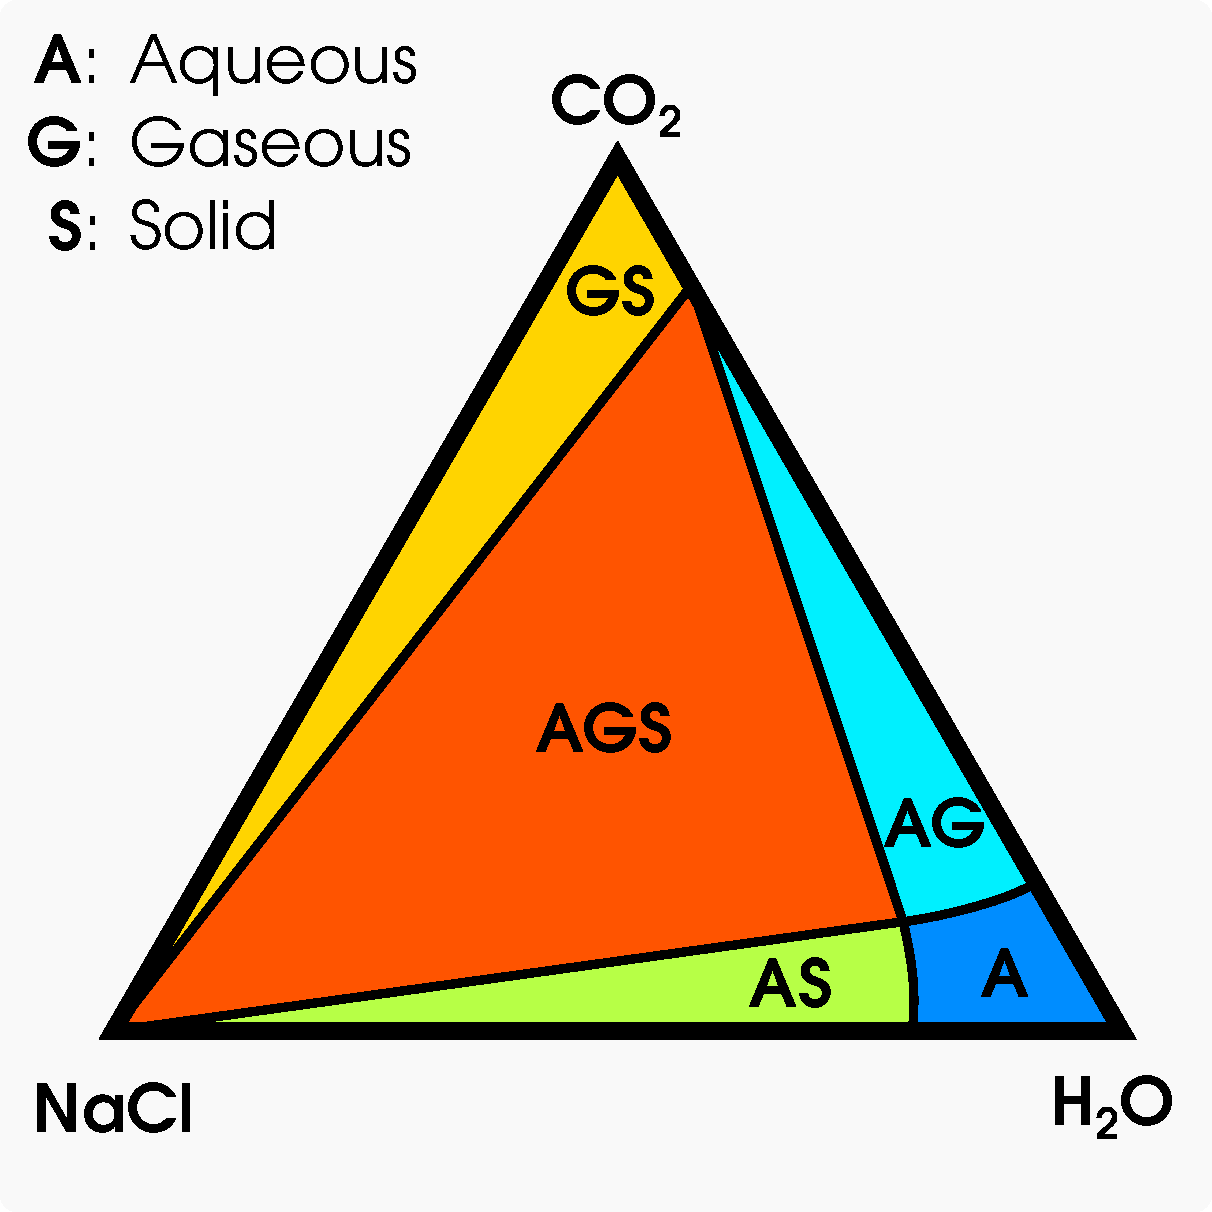
\includegraphics[width=0.9\columnwidth]{figures/applications/ternary-phase-diagram-h2o-co2-nacl}
\caption*{Ternary phase diagram.}
\end{figure}

\ecol
\end{frame}
%
% --------------------------------------------------------------------------------------------------------------------%
% Final considerations about defining the chemical system
% --------------------------------------------------------------------------------------------------------------------%
%
\begin{frame}{Final considerations about defining the chemical system}
	\vskip 10pt
\begin{itemize}
\item In most computer codes for modeling geochemical reactions, no manual
selection of phases and species are needed. 
\pause
\item These can be determined \textbf{automatically} by searching in \textbf{thermodynamic
databases} all possible species and phases that could exist for a
given model input. 
\pause
\item Depending on the available database, you can model different things: 
\begin{itemize}
\item supcrt98.xml
\item supcrt98-organics.xml (includes organic species)
\item thermofun.json (T = 200 °C, critical temperatures and pressures of gases used in Peng-Robinson's EOS) 
\item ColdChem.dat (a low-temperature aqueous thermodynamic model)
\end{itemize}

\end{itemize}
\end{frame}
